% SVN Info:
% $Date: 2020-11-25 15:16:56 +0100 (Mi, 25 Nov 2020) $
% $Rev: 5261 $
% $Author: kolja $
\documentclass[10pt,notitlepage]{scrreprt}
%
\usepackage[utf8]{inputenc}
\usepackage[T1]{fontenc}
\usepackage{fontspec}
\usepackage[usenames, dvipsnames]{color}
\usepackage{svg}
\usepackage{graphicx} %for including figures
\usepackage{tabularx}
\usepackage{amsmath} %for math environments
\usepackage{wrapfig}

\usepackage[%showframe,
left=25mm, right=25mm, top=24mm, bottom=24mm]{geometry} %for page properties (pagestyle)


\usepackage[section,subsection,subsubsection]{extraplaceins} %for binding figures to a (sub-)section
\usepackage{listings}%for code in latex document
\usepackage{textcomp}%for code in latex document
\usepackage{fancyhdr}%for header, footer
\usepackage{balance}%for two-column layout
\usepackage[colorlinks=true,linkcolor=cronblue,urlcolor  = gry]{hyperref}
\usepackage{array} %for centered AND constant width columns
\usepackage{longtable}
\usepackage{siunitx}
%
\fancyfoot[C,CO]{\thepage} %sets footer
\fancyfoot[L,LO]{\fontsize{17}{2}\selectfont
\sffamily \textcolor{gry}{~\url{www.cronologic.de}}} %sets footer

%%%Revision, also update Ndigo_UGRev.tex
\fancyfoot[R,RO]{Ndigo5G User Guide \hyperlink{ugrev}{1.2.3rc}} %sets footer

\pagestyle{fancy}
\fancyhead{} %removes header
\renewcommand{\headrulewidth}{0pt} %removes header line
\renewcommand{\footrulewidth}{1pt} %creates footer line
\renewcommand{\footrule}{{\color{cronblue}%
\vskip-\footruleskip\vskip-\footrulewidth
\hrule width\headwidth height\footrulewidth\vskip\footruleskip}}


%%% set fonts and colors according to CI styleguide
\definecolor{lbcolor}{gray}{0.9} % background of code listings
\definecolor{crongrey}{gray}{0.32} %Variablendeklaration API

\newfontfamily\chapterfont{TeX Gyre Adventor}
\addtokomafont{chapter}{\fontsize{19pt}{12}\selectfont\color{cronorange}\chapterfont\bfseries }
\newfontfamily\sectionfont{Montserrat}
\addtokomafont{section}{\fontsize{14pt}{12}\selectfont\color{cronorange}\sectionfont\bfseries}
\newfontfamily\subsectionfont{Montserrat}
\addtokomafont{subsection}{\fontsize{12pt}{12}\selectfont\color{cronblue}\subsectionfont \bfseries}
\newfontfamily\subsubsectionfont{Montserrat}
\addtokomafont{subsubsection}{\fontsize{12pt}{12}\selectfont\color{cronblue}\subsubsectionfont \bfseries}
\addtokomafont{caption}{\sectionfont\fontsize{12pt}{12}\selectfont\color{crongrey}}  %font of caption
\addtokomafont{captionlabel}{\sectionfont\fontsize{12pt}{12}\selectfont\color{crongrey}}  


\newcommand{\cronvar}[2]{\noindent\textsf{\textbf{\textcolor{crongrey}{#1} #2}}}%for variable declaration
\newcommand{\crondef}[1]{\noindent\textsf{\textcolor{crongrey}{\#{}define} #1}}%for definitions
\newcommand{\tu}{\textunderscore}%shorter
\newcommand{\subscript}[1]{\ensuremath{_{\textrm{#1}}}}
\renewcommand{\arraystretch}{1.6}
%
\parskip 8pt

%\DeclareTextFontCommand{\textmyfont}{texgyreadventor-bold.otf}
\usepackage{efbox}
%%%%%%%%%%%%%%%%%%%%
%\usepackage{graphicx}
\usepackage{tikz}
\usepackage{xcolor}
\usepackage{montserrat} %% Option 'defaultfam'
%% only if the base font of the document is to be sans serif
\usepackage[T1]{fontenc}
\renewcommand*\oldstylenums[1]{{\fontfamily{Montserrat-TOsF}\selectfont #1}}

\addtokomafont{disposition}{\chapterfont\color{cronorange}}

\usepackage{hologo}

\definecolor{org}{RGB}{237,120,0}
\definecolor{gry}{RGB}{ 157,157,156}
\definecolor{crongrey}{gray}{0.5} %Variablendeklaration API
\definecolor{cronorange}{RGB}{237, 120, 0}
\definecolor{cronblue}{RGB}{55, 110, 181}
\definecolor{cronblack}{RGB}{0,0,0}
\newcommand{\codeexamplesize}{\footnotesize}

\setmonofont{texgyreadventor-bold}[
    Scale=0.85,
    Extension = .otf
    ]

    \usepackage[most]{tcolorbox}

%%%%%%%%%%%%%%%%%%%%%%%%%%%%%%%%%%%%
\usepackage{float}
\usepackage{efbox,graphicx}
\efboxsetup{linecolor=gray!50,linewidth=0.5pt}
%%%%%%%%%%%%%%%%%%%%%%%%%
    \usepackage{setspace}
    \usepackage{caption}
    \usepackage{tocloft}


%% for TOC
\renewcommand{\cftchapfont}{\fontsize{12}{12}\selectfont\bfseries}
\renewcommand{\cftsecfont}{\fontsize{12}{12}\selectfont}     
\renewcommand{\cftsubsecfont}{\fontsize{12}{12}\selectfont}        % \subsection font in ToC
\renewcommand{\cftsubsubsecfont}{\fontsize{12}{12}\selectfont}


\renewcommand{\familydefault}{\sfdefault}

\color{cronblack}\setstretch{1.08} 
%%%%%%%%%%%%%%%%%%%%%%%%%%%

\begin{document}
\thispagestyle{empty}
\begin{tikzpicture}
\draw[inner sep=0pt] node at (0,0)   { 
\includegraphics[width=155mm]{figures/cronologic.pdf}};
\end{tikzpicture}

\begin{minipage}{0.83\textwidth}
\begin{tabular}{l}


\begin{tikzpicture}
\draw[inner sep=0pt] node at (-8.1,1){\fontsize{20}{2}\selectfont
\sectionfont 
{\textcolor{org}{Ndigo5G-PCIe}}};

\draw[align=center] node at (-8.3,0){\fontsize{20}{2}\selectfont
\sffamily \textcolor{org}{USER GUIDE}};
\end{tikzpicture}
\\ \vspace{5pt}
%{\efbox{
%\hspace{-10pt}
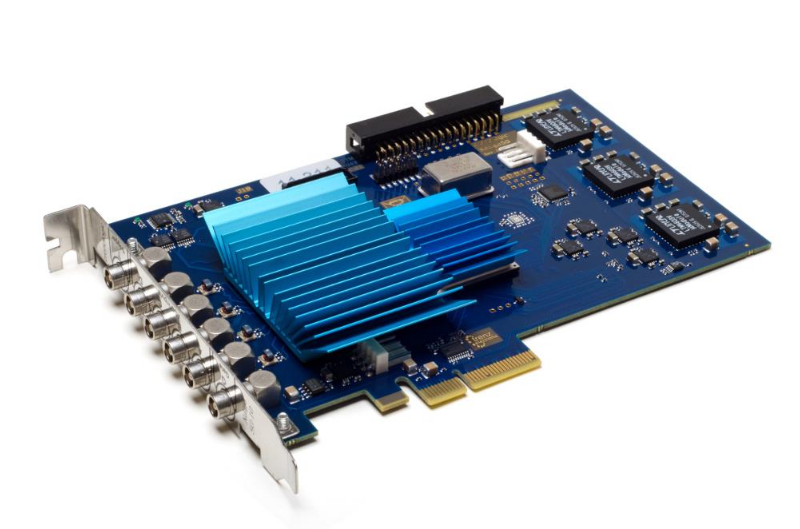
\includegraphics[width=120mm,height=150mm,keepaspectratio]{figures/Title5G.pdf}
%}}
\\
\end{tabular}
\end{minipage}
\begin{minipage}{0\textwidth}
\vspace{25pt}

\begin{tikzpicture}
\draw[inner sep=0pt] node at (0,-5){ 
\fontsize{80}{2}\selectfont
\ttfamily \textcolor{org}{ \rotatebox{90}{Ndigo5G-PCIe}}};
\end{tikzpicture}
\end{minipage}

\vspace{-25pt}
\begin{minipage}{0\textwidth}

\begin{tikzpicture}
\draw[inner sep=0pt] node at (-3,-18){\fontsize{20}{2}\selectfont
\sffamily \textcolor{gry}{~\url{www.cronologic.de}}};
\end{tikzpicture}
\end{minipage}
\newpage


\newgeometry{left=25mm, right=25mm, top=25mm, bottom=25mm}
 \newpage 
%	\maketitle
	\thispagestyle{empty}
	\newpage
	\pagenumbering{roman}
	\tableofcontents
	\clearpage
	\pagestyle{fancy}
	\pagenumbering{arabic}
	\chapter{Introduction}
		% SVN Info:
% $Date: 2019-06-04 12:35:07 +0200 (Di, 04 Jun 2019) $
% $Rev: 4976 $
% $Author: andreas $
The Ndigo5G is a digitizer and transient recorder designed to sample relatively shorts pulses in rapid repetition. It produces a stream of output packets, each containing data from a single trigger event together with a timestamp.
\section{Features}
	\begin{itemize}
		\item 10 bit dynamic range
		\item up to 5 Gsps sample rate (in 1 channel mode)
		\item up to four ADC channels
		\item digital TDC input that can also be used for gating and triggering
		\item 2\textsuperscript{nd} digital input for gating or triggering
		\item PCIe 4x 1.1 with 800 MB/s throughput
		\item possibility to synchronize multiple boards
		\item extension board with four additional digital inputs
	\end{itemize}
	\chapter{Hardware}
		\input{Ndigo_Hardware.tex}
	\chapter{Driver Programming API}
		% SVN Info:
% $Date: 2019-06-04 16:01:22 +0200 (Di, 04 Jun 2019) $
% $Rev: 4980 $
% $Author: andreas $
The API is a DLL with C linkage. The functions provided by the DLL are declared in \textsf{Ndigo\tu interface.h}. \par

\section{Constants}

    \crondef{NDIGO\tu CHANNEL\tu COUNT 4}\\
    The number of analog input channels.\par

    \crondef{NDIGO\tu GATE\tu COUNT 4}\\
    The number of gating blocks.\par

    \crondef{NDIGO\tu TRIGGER\tu COUNT 16}\\
    The number of triggers. Two per analog input, one per digital input plus some specials.\par

    \crondef{NDIGO\tu ADD\tu TRIGGER\tu COUNT 6}\\
    Additional set of triggers for digital inputs.

    \section{Initialization}

        \cronvar{int}{ndigo\tu count\tu devices(}\cronvar{int}{*error\tu code}, \cronvar{char}{**error\tu message)}\\
        Return the number of boards that are supported by this driver in the system.\par

        \cronvar{int}{ndigo\tu get\tu default\tu init\tu parameters(}\cronvar{ndigo\tu init\tu parameters}{*init)}\\
        Get a set of default parameters to feed into \textsf{ndigo\tu init()}. This must always be used to initialize the \textsf{ndigo\tu init\tu parameter structure}.\par

        \cronvar{ndigo\tu device}{*ndigo\tu init(}\cronvar{ndigo\tu init\tu parameters}{*params}, \cronvar{int}{*error\tu code},\newline \cronvar{char}{**error\tu message)}\\
        Open and initialize the Ndigo board with the given index. With \textsf{error\tu code} and \textsf{error\tu message} the user must provide pointers to buffers where error information should be written by the driver. The buffer for the error message must by at least 80 chars long.\par

        \textsf{params} is a structure of type \textsf{ndigo\tu init\tu parameters} that must be completely initialized.\par

        \cronvar{int}{ndigo\tu close(}\cronvar{ndigo\tu device}{*device)}\\
        Finalize the driver for this device.

        \subsection{Structure ndigo\tu init\tu parameters}

            \cronvar{int}{version}\\
            Must be set to \textsf{NDIGO\tu API\tu VERSION}\par

            \cronvar{int}{card\tu index}\\
            The index in the list of Ndigo5G boards that should be initialized. There might be multiple boards in the system that are handled by this driver as reported by \textsf{ndigo\tu count\tu devices}. This index selects one of them. Boards are enumerated depending on the PCIe slot. The lower the bus number and the lower the slot number the lower the card index.\par

            \cronvar{int}{board\tu id}\\
            This 8-bit number is filled into each packet created by the board and is useful if data streams of multiple boards will be merged. If only Ndigo5G cards are used this number can be set to the card index. If boards of different types that use a compatible data format are used in a system each board should get a unique ID. Can be changed with \textsf{int ndigo\tu set\tu board\tu id(ndigo\tu device *device, int board\tu id)}.\par

            \cronvar{ndigo\tu bool\tu t}{use\tu external\tu clock}\\
            Use 10MHz clock supplied by IPC flat band cable. Must be set for all slaves.\par

            \cronvar{ndigo\tu bool\tu t}{drive\tu external\tu clock}\\
            Drive internal 10MHz clock of this board to IPC flat band cable. Must be set for master.\par

            \cronvar{ndigo\tu bool\tu t}{is\tu slave}\\
            Data acquisition of this board is controlled by the master board.\par

            \cronvar{int}{sync\tu period}\\
            Period of the multi-card sync pulse. Should be set to 4 (default) when using several Ndigo boards in sync. Ignored for single board setups. The Ndigo5G has 4 phases relative to the global 10MHz clock.\par

            \cronvar{int}{sync\tu delay}\\
            Fine tap delay for incoming sync signals.\par

            \cronvar{ndigo\tu bool\tu t}{force\tu window\tu calibration}\\
            If true/1, valid data window is detected at initialization. Default value is false/0: values from flash memory are used in order to set data window to correct position.

            \cronvar{ndigo\tu bool\tu t}{hptdc\tu sync\tu enabled}\\
            A HPTDC is connected to this board. Enables the clock and sync line from the Ndigo5G to the HPTDC.\par

            \cronvar{\tu \tu int64}{buffer\tu size[8]}\\
            The minimum size of the DMA buffer. If set to 0 the default size of 16MByte is used. Ndigo5G only uses \textsf{buffer\tu size[0]}.\par

            \cronvar{int}{buffer\tu type}\\
            Must be set to \textsf{NDIGO\tu BUFFER\tu ALLOCATE}.\par

            \cronvar{\tu \tu int64}{buffer\tu address}\\
            Ignored. Might be used for future buffer types.\par

            \cronvar{int}{variant}\\
            Set to 0. Can be used to activate future device variants such as different base frequencies.\par

            \cronvar{int}{device\tu type}\\
            Initialized by \textsf{ndigo\tu get\tu default\tu init\tu parameters()}. Must be left unchanged.

            \begin{description}
                \item[] \crondef{CRONO\tu DEVICE\tu HPTDC 0}
                \item[] \crondef{CRONO\tu DEVICE\tu NDIGO5G 1}
                \item[] \crondef{CRONO\tu DEVICE\tu NDIGO250M 2}
            \end{description}

            \cronvar{int}{dma\tu read\tu delay}\\
            Initialized by \textsf{ndigo\tu get\tu default\tu init\tu parameters()}. The write-pointer update is delay by this number of 4\,ns clock periods to hide race conditions between software and DMA.

    \clearpage
    \section{Status Information}
        \subsection{Functions for Information Retrieval}

            The driver provides functions to retrieve detailed information on the type of board, its configuration, settings and state. The information is split according to its scope and the computational requirements to query the information from the board.\par

            \cronvar{int}{ndigo\tu get\tu driver\tu revision()}\\
            Returns the driver version, same format as ndigo\tu static\tu info::driver\tu revision. This function does not require a
            present Ndigo5G device.

            \cronvar{const char*}{ndigo\tu get\tu driver\tu revision\tu str()}\\
            Returns the driver version including SVN build revision as a string. This function does not require a
            present Ndigo5G device.

            \cronvar{int}{ndigo\tu get\tu static\tu info(}\cronvar{ndigo\tu device}{*device},\cronvar{ndigo\tu static\tu info}{*info)}\\
            This structure contains information about the board that does not change during run time.\par

            \cronvar{int}{ndigo\tu get\tu param\tu info(}\cronvar{ndigo\tu device}{*device}, \cronvar{ndigo\tu param\tu info}{*info)}\\
            The structure returned by this call contains information that changes indirectly due to configuration changes.\par

            \cronvar{int}{ndigo\tu get\tu fast\tu info(}\cronvar{ndigo\tu device}{*device}, \cronvar{ndigo\tu fast\tu info}{*info)}\\
            This call returns a structure that contains dynamic information that can be obtained within a few microseconds.\par

            \cronvar{int}{ndigo\tu get\tu slow\tu info(}\cronvar{ndigo\tu device}{*device}, \cronvar{ndigo\tu slow\tu info}{*info)}\\
            The data reported in this structure requires milliseconds to be obtained. The application should only call it in situation where the program flow can cope with an interruption of that magnitude.

        \cronvar{const char*}{ndigo\tu get\tu last\tu error\tu message(}\cronvar{ndigo\tu device}{*device)}\\
        \subsection{Structure ndigo\tu static\tu info}

            This structure contains information about the board that does not change during run time. It is provided by the function \textsf{ndigo\tu get\tu static\tu info}.\par

            \cronvar{int}{size}\\
            The number of bytes occupied by the structure\par

            \cronvar{int}{version}\\
            A version number that is increased when the definition of the structure is changed. The increment can be larger than one to match driver version numbers or similar. Set to 0 for all versions up to first release.\par

            \cronvar{int}{board\tu id}\\
            Index of the board as passed to the constructor or set via \textsf{int ndigo\tu set\tu board\tu id(ndigo\tu device *device, int board\tu id)}.\par

            \cronvar{int}{driver\tu revision}\\
            The lower three bytes contain a triple level hierarchy of version numbers, e.g. 0x010103 encodes version 1.1.3.\par

            A change in the first digit generally requires a recompilation of user applications. Change in the second digit denote significant improvements or changes that don't break compatibility and the third digit changes with minor bug fixes and similar updates.\par

            \cronvar{int}{firmware\tu revision}\\
            Firmware revision of the FPGA configuration. This increments only when there is a functional change.\par

            \cronvar{int}{board\tu revision}\\
            0 for experimental prototypes labeled ``Rev. 1''\\
            2 for the version produced until 2010 labeled ``Rev. 2''`\\
            3 for the version produced starting in 2011 labeled ``Rev. 3''\\

            \cronvar{int}{board\tu configuration}\\
            Describes the schematic configuration of the board.\par

            \noindent\textit{For board revision 0 this always reads 0.}\par

            \noindent\textit{For board revision 2 the following assignments are valid:}\par

            \noindent If Bit 3 = 0 this following is valid:\\
            Bit 0 determines the ADC resolution. ($0 = 8-\text{bit}$ or $1 = 10-\text{bit}$).\\
            Bit 1 determines whether the TDC-oscillator is present ($0 = \text{oscillator present}$, $1 = \text{simple trigger}$).\\
            Bit 2 determines the input connectors ($0 = \text{single ended}$, $1 = \text{differential}$).\par

            \noindent Bit $3 = 1$ signifies a special version of the board\\
            0xA is Ndigo1250M-12 single ended with digital trigger\\
            0x8 is Ndigo5G-8 single ended with digital trigger\par

            \noindent\textbf{For Board revision 3 the following assignments are valid:}\par

            \noindent Bit 2 determines the input connectors ($0 = \text{single ended}$, $1 = \text{differential}$).\par

            \noindent The other bits have one of the following patterns [Bits 3...0]\par

            \noindent 0010 Ndigo5G-10 2.5u 10\\
            0011 Ndigo5G-8-AQ 2.5u 8\\
            0110 Ndigo5G-10-Diff 560pF 10 DIFF\\
            1000 Ndigo5G-8 560pF 8+\\
            1010 Ndigo1250M-12 2.2uF 12 S DC\\
            1011 Ndigo5G-10 560pF 10\\
            1110 Ndigo5G-S 2.2uF 10 S Infiniband, DIFF\\
            1111 Ndigo5G-R = fADC4/10 560pF 10\par

            \cronvar{int}{adc\tu resolution}\\
            Number of bits of the ADC, set to 0 if unknown.\par

            \cronvar{double}{nominal\tu sample\tu rate}\\
            Sample rate in once channel mode. Usually $5.0e9 = 5 Gsps$.\par

            \cronvar{double}{analog\tu bandwidth}\\
            9.5e8 for \SI{950}{\MHz}.

            \cronvar{int}{chip\tu id}\\
            16 bit factory ID of the ADC chip\par

            \cronvar{int}{board\tu serial}\\
            Serial number with the year minus 2000 in the highest 8 bits of the integer and a running number in the lower 24 bits. This number is identical with the one on the label on the board.\par

            \cronvar{int}{flash\tu serial\tu low}\\
            \cronvar{int}{flash\tu serial\tu high}\\
            64 bit manufacturer serial number of the flash chip.\par

            \cronvar{int}{flash\tu valid}\\
            If not 0 the driver found valid calibration data in the flash on the board and is using it.\par

            \cronvar{ndigo\tu bool\tu t}{dc\tu coupled}\\
            Returns false for the standard AC coupled Ndigo5G.\par

            \cronvar{int}{subversion\tu revision}\\
            A number to track builds of the firmware in more detail than the firmware revision. It changes with every change in the firmware, even if there is no visible effect for the user.\par

            \cronvar{char}{calibration\tu date[20]}\\
            DIN EN ISO 8601 string YYYY-MM-DD HH:DD describing the time when the card was calibrated.

        \subsection{Structure ndigo\tu param\tu info}

            \cronvar{int}{size}\\
            The number of bytes occupied by the structure.\par

            \cronvar{int}{version}\\
            A version number that is increased when the definition of the structure is changed. The increment can be larger than one to match driver version numbers or similar. Set to 0 for all versions up to
first release.\par

            \cronvar{double}{bandwidth}\\
            Bandwidth setting of the ADC. Note: This is \emph{not} the bandwidth of the analog board frontend. \par

            \cronvar{double}{sample\tu rate}\\
            Sample rate. This is 1.25e9, 2.5e9 or 5.0e9 depending on the current ADC mode. $\text{sample\tu rate}\cdot \text{channels} = 5.0e9$.\par

            \cronvar{double}{sample\tu period}\\
            The period one sample in the data represents in picoseconds\par

            \cronvar{int}{board\tu id}\\
            The number the board uses to identify the data source in the output data stream.\par

            \cronvar{int}{channels}\\
            Number of channels. 1, 2 or 4 depending on the ADC mode chosen. $\text{sample\tu rate}\cdot\text{channels} = 5.0e9$.\par

            \cronvar{int}{channel\tu mask}\\
            Mask with a set bit for each enabled input channel.\par

            \cronvar{\tu\tu int64}{total\tu buffer}\\
            The total amount of the DMA buffer in bytes.\par

%			\cronvar{\tu\tu int64}{free\tu buffer}\\
%			Unused portion of the DMA buffer in bytes.\par

        \subsection{Structure ndigo\tu fast\tu info}

            \cronvar{int}{size}\\
            The number of bytes occupied by the structure\par

            \cronvar{int}{version}\\
            A version number that is increased when the definition of the structure is changed. The increment can be larger than one to match driver version numbers or similar. Set to 0 for all versions up to first release.\par

            \cronvar{int}{adc\tu rpm}\\
            Speed of the ADC fan. Reports 0 if no fan is present.\par

            \cronvar{int}{fpga\tu rpm}\\
            Speed of the FPGA fan. Reports 0 if no fan is present.\par

            \cronvar{int}{alerts}\\
            Alert bits from the system monitor.\par

            \noindent Bit 0 : FPGA temperature alert ($> 85^{\circ}C$)\\
            Bit 1 : Internal FPGA voltage out of range ($< 1.01V$ or $> 1.08V$)\\
            Bit 2 : FPGA auxiliary voltage out of range. ($< 2.375V$ or $>  2.625V$)\\
            Bit 3 : FPGA temperature critical ($> 125^{\circ}C$)\\
            Bit 4 : ADC temperature alert ($> 90^{\circ}C$)\\
            Bit 5 : ADC temperature critical ($> 100^{\circ}C$): will automatically be turned off.\par

            \cronvar{double}{voltage\tu aux}\\
            Auxiliary FPGA voltage, nominal 2.5V\par

            \cronvar{double}{voltage\tu int}\\
            Internal FPGA voltage, nominal 1.0V\par

            \cronvar{double}{fpga\tu temperature}\\
            In $^\circ$C measured on die.\par

            \cronvar{int}{pcie\tu link\tu width}\\
            Number of PCIe lanes that the card uses. Should be 4 for Ndigo5G. \par

            \cronvar{int}{pcie\tu max\tu payload}\\
            Maximum size in bytes for one PCIe transaction, depends on system configuration.\par

        \subsection{Structure ndigo\tu slow\tu info}

            \cronvar{int}{size}\\
            The number of bytes occupied by the structure.\par

            \cronvar{int}{version}\\
            A version number that is increased when the definition of the structure is changed. The increment can be larger than one to match driver version numbers or similar. Set to 0 for all versions up to
first release.\par

            \cronvar{double}{adc\tu temperature}\\
            ADC temperature in $^{\circ}C$ measured on die.\par

            \cronvar{double}{board\tu temperature}\\
            In $^{\circ}C$.

    \section{Configuration}

        The device is configured with a configuration structure. The user should first obtain a structure that contains the default settings of the device read from an on-board ROM, then modify the structure as needed for the user application and use the result to configure the device.\par

        \cronvar{int}{ndigo\tu get\tu default\tu configuration(}\cronvar{ndigo\tu device}{*device,}\newline \cronvar{ndigo\tu configuration}{*config)}\par

        \cronvar{int}{ndigo\tu get\tu current\tu configuration(}\cronvar{ndigo\tu device}{*device,}\newline \cronvar{ndigo\tu configuration}{*config)}\par

        \cronvar{int}{ndigo\tu configure(}\cronvar{ndigo\tu device} {*device,} \cronvar{ndigo\tu configuration}{*config)}\par

        \cronvar{int}{ndigo\tu set\tu board\tu id(}\cronvar{ndigo\tu device}{*device,} \cronvar{int}{board\tu id)}\\
        The \textsf{board\tu id} can be changed after initialization of the card. If cronotools are used the \textsf{board\tu id} changes have to be done before cronotools initialization.

        \subsection{Structure ndigo\tu configuration}

            This is the structure containing the configuration information. It is used in conjunction with \textsf{ndigo\tu get\tu default\tu configuration}, \textsf{ndigo\tu get\tu current\tu configuration} and \textsf{ndigo\tu configure}.\par

            It uses internally the structures \textsf{ndigo\tu trigger\tu block} and \textsf{ndigo\tu trigger}.\par

            \cronvar{int}{size}\\
            The number of bytes occupied by the structure.\par

            \cronvar{int}{version}\\
            A version number that is increased when the definition of the structure is changed. The increment can be larger than one to match driver version numbers or similar. Set to 0 for all versions up to first release.\par

            \cronvar{int}{reserved1}\\
            Reserved for internal usage. Do not change.\par

            \cronvar{int}{adc\tu mode}\\
            Constant describing the ADC mode\par

            \crondef{NDIGO\tu ADC\tu MODE\tu ABCD 0}\\
            \crondef{NDIGO\tu ADC\tu MODE\tu AC 4}\\
            \crondef{NDIGO\tu ADC\tu MODE\tu BC 5}\\
            \crondef{NDIGO\tu ADC\tu MODE\tu AD 6}\\
            \crondef{NDIGO\tu ADC\tu MODE\tu BD 7}\\
            \crondef{NDIGO\tu ADC\tu MODE\tu A 8}\\
            \crondef{NDIGO\tu ADC\tu MODE\tu B 9}\\
            \crondef{NDIGO\tu ADC\tu MODE\tu C 10}\\
            \crondef{NDIGO\tu ADC\tu MODE\tu D 11}\\
            \crondef{NDIGO\tu ADC\tu MODE\tu AAAA 12}\\
            \crondef{NDIGO\tu ADC\tu MODE\tu BBBB 13}\\
            \crondef{NDIGO\tu ADC\tu MODE\tu CCCC 14}\\
            \crondef{NDIGO\tu ADC\tu MODE\tu DDDD 15}\\
            \crondef{NDIGO\tu ADC\tu MODE\tu A12 28} // not available on all boards\\
            \crondef{NDIGO\tu ADC\tu MODE\tu B12 29} // not available on all boards\\
            \crondef{NDIGO\tu ADC\tu MODE\tu C12 3}0 // not available on all boards\\
            \crondef{NDIGO\tu ADC\tu MODE\tu D12 31} // not available on all boards\par

            \cronvar{double}{bandwidth}\\
            Set to the minimum bandwidth required for the application. Lower bandwidth results in reduced noise. The driver will set the ADC to the minimum setting that has at least the desired bandwidth and report the selected bandwidth in the \textsf{ndigo\tu param\tu info} structure. The -8, -10 and -12 versions currently supports 1GHz and 3GHz bandwidth, the -8AQ version supports 2GHz, 1.5GHz, 600MHz and 500 MHz. The bandwidth of the analog frontend of the board remains unchanged at about 950\,MHz.
            \par

            \cronvar{ndigo\tu bool\tu t}{reserved}\\
            \cronvar{ndigo\tu bool\tu t}{tdc\tu enabled}\\
            Enable capturing of TDC measurements on external digital input channel.\par

            \cronvar{ndigo\tu bool\tu t}{tdc\tu fb\tu enabled}\\
            Enable enhanced TDC resolution. Currently not implemented.\par

            \cronvar{double}{analog\tu offset[NDIGO\tu CHANNEL\tu COUNT]}\\
            Sets the input DC offset-values to plus/minus this value in volts. Defaults to 0.\par

            \cronvar{double}{dc\tu offset[2]}\\
            Sets the DC offset in volts for the TDC trigger input (index 1) and the GATE input (index 0). The default is -0.35 which is a good setting vor \SI{0.8}{\volt} negative NIM pulses.
            The values are limited by the driver to the range [-1.25, 1.25]. When using the TDC, nonnegative values for index 1 throw an error. \par

            \cronvar{ndigo\tu trigger}{trigger[NDIGO\tu TRIGGER\tu COUNT + NDIGO\tu ADD\tu TRIGGER\tu COUNT]}\\
            Configuration of the external trigger sources. Threshold is ignored for entries 8 and above.\par

            The trigger indexes refer to the entry in the trigger array and are defined like this:\par

            \crondef{NDIGO\tu TRIGGER\tu A0 0}\\
            \crondef{NDIGO\tu TRIGGER\tu A1 1}\\
            \crondef{NDIGO\tu TRIGGER\tu B0 2}\\
            \crondef{NDIGO\tu TRIGGER\tu B1 3}\\
            \crondef{NDIGO\tu TRIGGER\tu C0 4}\\
            \crondef{NDIGO\tu TRIGGER\tu C1 5}\\
            \crondef{NDIGO\tu TRIGGER\tu D0 6}\\
            \crondef{NDIGO\tu TRIGGER\tu D1 7}\\
            \crondef{NDIGO\tu TRIGGER\tu TRIGGER 8}\\
            \crondef{NDIGO\tu TRIGGER\tu TDC 8}\\
            \crondef{NDIGO\tu TRIGGER\tu GATE 9}\\
            \crondef{NDIGO\tu TRIGGER\tu BUS0 10}\\
            \crondef{NDIGO\tu TRIGGER\tu BUS1 11}\\
            \crondef{NDIGO\tu TRIGGER\tu BUS2 12}\\
            \crondef{NDIGO\tu TRIGGER\tu BUS3 13}\par

            \crondef{NDIGO\tu TRIGGER\tu AUTO 14}\\
            \crondef{NDIGO\tu TRIGGER\tu ONE 15}\par

            Always positive edge-sensitive sources:\\
            \crondef{NDIGO\tu TRIGGER\tu TDC\tu PE 16}\\
            \crondef{NDIGO\tu TRIGGER\tu GATE\tu PE 17}\\
            \crondef{NDIGO\tu TRIGGER\tu BUS0\tu PE 18}\\
            \crondef{NDIGO\tu TRIGGER\tu BUS1\tu PE 19}\\
            \crondef{NDIGO\tu TRIGGER\tu BUS2\tu PE 20}\\
            \crondef{NDIGO\tu TRIGGER\tu BUS3\tu PE 21}\par

            \cronvar{ndigo\tu trigger\tu block}{trigger\tu block[NDIGO\tu CHANNEL\tu COUNT + 1]}\\
            A structure describing the trigger settings of the four channels plus the timestamp channel. In some modes not all channels are used.\par

            \cronvar{ndigo\tu gating\tu block}{gating\tu block[4]}\\
            A structure describing the gating blocks that can be used by the trigger blocks to filter triggers.\par

            \cronvar{ndigo\tu extension\tu block}{extension\tu block[NDIGO\tu EXTENSION\tu COUNT]}\\
            A structure describing the routing of the 4 digital channels of the Ndigo extension board to the trigger matrix.\par

            \cronvar{int}{drive\tu bus[4]}\\
            Enable output drive for each of the four external sync lines. Each integer represents a bitmask selecting the trigger sources for that line. The bit mapping is described in section ``Structure \textsf{ndigo\tu trigger\tu block}'' on page \pageref{cp:triggerblock}.\par

            \cronvar{int}{auto\tu trigger\tu period}\\
            \cronvar{int}{auto\tu trigger\tu random\tu exponent}\\
            Create a trigger either periodically or randomly. There are two parameters $M = \text{trigger\tu period}$ and $N = \text{random\tu exponent}$ that result in a distance between triggers of

            \begin{align}
                T = M + [1...2^N] - 1
            \end{align}

            clock cycles.

            \begin{align}
                8 &\leq M < 2^{32}\\
                0 &\leq N < 32
            \end{align}

            There is no enable or reset as the usage of this trigger can be configured in the trigger block channel source field.\par

            \cronvar{int}{output\tu mode}\\
            Defines the data representation in the output. Signed16 scales and INL-corrects the input. RAW directly presents the ADC values.\par

            \crondef{NDIGO\tu OUTPUT\tu MODE\tu SIGNED16 0}\\
            \crondef{NDIGO\tu OUTPUT\tu MODE\tu RAW 1}\\
            \crondef{NDIGO\tu OUTPUT\tu MODE\tu CUSTOM 2}\\
            \crondef{NDIGO\tu OUTPUT\tu MODE\tu CUSTOM\tu INL 3}\par

            \cronvar{lut\tu func}{custom\tu lut}\\
            If the \textsf{output\tu mode} is set to \textsf{NDIGO\tu OUTPUT\tu MODE\tu CUSTOM} or\\\textsf{NDIGO\tu OUTPUT\tu MODE\tu CUSTOM\tu INL} this function is used for mapping from ADC value to output value. The driver will call this function with a value from -1 to +1 and the function must return the corresponding signed 16 bit value that the board should return for an input voltage relative to the full scale range.\par

            \cronvar{typedef short}{(*lut\tu func)(}\cronvar{int}{channel,} \cronvar{float}{x)}\par

            This can be used, e.g., for custom INL, offset and gain correction that covers user front end electronics. It can also invert the signal or correct the effect of logarithmic input amplifiers etc.\par

            The LUT is applied on the board, thus using it does not cause any additional CPU load. In the mode ``\textsf{NDIGO\tu OUTPUT\tu MODE\tu CUSTOM\tu INL}'' the on-board INL correction table is applied before the user function, while ``\textsf{NDIGO\tu OUTPUT\tu MODE\tu CUSTOM}'' does not perform INL correction. In order to use the user lookup table functionality \textsf{lut\tu func} must be set to a pointer to the LUT-function.

        \subsection{Structure ndigo\tu trigger}

            \cronvar{short}{threshold}\\
            Sets the threshold for the trigger block within the range of the ADC data of -32768 and +32768.\par

            For trigger indices \textsf{NDIGO\tu TRIGGER\tu TDC} to \textsf{NDIGO\tu TRIGGER\tu BUS3\tu PE} the threshold is ignored.\par

            \cronvar{ndigo\tu bool\tu t}{edge}\\
            If set this trigger implements edge trigger functionality else this is a level trigger.\par

            For trigger indices \textsf{NDIGO\tu TRIGGER\tu AUTO} and \textsf{NDIGO\tu TRIGGER\tu ONE} this is ignored.\par

            For trigger indices \textsf{NDIGO\tu TRIGGER\tu TDC\tu PE} to \textsf{NDIGO\tu TRIGGER\tu BUS3\tu PE} this must be set.\par

            \cronvar{ndigo\tu bool\tu t}{rising}\\
            If set trigger on rising edges or when above threshold.\par

            For trigger indices \textsf{NDIGO\tu TRIGGER\tu AUTO} and \textsf{NDIGO\tu TRIGGER\tu ONE} this is ignored.\par

            For trigger indices \textsf{NDIGO\tu TRIGGER\tu TDC\tu PE} to \textsf{NDIGO\tu TRIGGER\tu BUS3\tu PE} this must be set.

        \subsection{Structure ndigo\tu trigger\tu block\label{cp:triggerblock}}

        \cronvar{ndigo\tu bool\tu t}{enabled}\\
        Activate triggers on this channel.\par

        \cronvar{ndigo\tu bool\tu t}{retrigger}\\
        If a new trigger condition occurs while the postcursor is acquired the packet is extended by starting a new postcursor. Otherwise, the new trigger is ignored and the packet ends after the precursor of the first trigger.\par

        The retrigger setting is ignored for the timestamp channel.\par

        \cronvar{ndigo\tu bool\tu t}{reserved1}\\
        Defaults to false. Do not change.\par

        \cronvar{ndigo\tu bool\tu t}{reserved2}\\
        Defaults to false. Do not change.\par

        \cronvar{int}{precursor}\\
        Precursor in multiples of 3.2ns. The amount of data preceding a trigger that is captured.\par

        The precursor setting is ignored for the timestamp channel.\par

        \cronvar{int}{length}\\
        In multiples of 3.2ns.\par

        The total amount of data that is recorded in addition to the trigger window. Precursor determines how many of these are ahead of the trigger and how many are appended after the trigger. In edge trigger mode the trigger window always is 3.2ns wide, in level trigger mode it is as long as the
trigger condition is fulfilled.\par

        The length setting is ignored for the timestamp channel.\par

        \cronvar{int}{sources}\\
        A bit mask with a bit set for all trigger sources that can trigger this channel.\par

        \begin{tabular}{lc}
            \crondef{NDIGO\tu TRIGGER\tu SOURCE\tu A0} & 0x00000001\\
            \crondef{NDIGO\tu TRIGGER\tu SOURCE\tu A1} & 0x00000002\\
            \crondef{NDIGO\tu TRIGGER\tu SOURCE\tu B0} & 0x00000004\\
            \crondef{NDIGO\tu TRIGGER\tu SOURCE\tu B1} & 0x00000008\\
            \crondef{NDIGO\tu TRIGGER\tu SOURCE\tu C0} & 0x00000010\\
            \crondef{NDIGO\tu TRIGGER\tu SOURCE\tu C1} & 0x00000020\\
            \crondef{NDIGO\tu TRIGGER\tu SOURCE\tu D0} & 0x00000040\\
            \crondef{NDIGO\tu TRIGGER\tu SOURCE\tu D1} & 0x00000080\\
            \crondef{NDIGO\tu TRIGGER\tu SOURCE\tu TDC} & 0x00000100\\
            \crondef{NDIGO\tu TRIGGER\tu SOURCE\tu GATE} & 0x00000200\\
            \crondef{NDIGO\tu TRIGGER\tu SOURCE\tu BUS0} & 0x00000400\\
            \crondef{NDIGO\tu TRIGGER\tu SOURCE\tu BUS1} & 0x00000800\\
        \end{tabular}\\
        \begin{tabular}{lc}
            \crondef{NDIGO\tu TRIGGER\tu SOURCE\tu BUS2} & 0x00001000\\
            \crondef{NDIGO\tu TRIGGER\tu SOURCE\tu BUS3} & 0x00002000
        \end{tabular}\\
        \begin{tabular}{lc}
            \crondef{NDIGO\tu TRIGGER\tu SOURCE\tu AUTO} & 0x00004000\\
            \crondef{NDIGO\tu TRIGGER\tu SOURCE\tu ONE} & 0x00008000
        \end{tabular}\\
        \begin{tabular}{lc}
            \crondef{NDIGO\tu TRIGGER\tu SOURCE\tu TDC\tu PE} & 0x01000000\\
            \crondef{NDIGO\tu TRIGGER\tu SOURCE\tu GATE\tu PE} & 0x02000000\\
            \crondef{NDIGO\tu TRIGGER\tu SOURCE\tu BUS0\tu PE} & 0x04000000\\
            \crondef{NDIGO\tu TRIGGER\tu SOURCE\tu BUS1\tu PE} & 0x08000000\\
            \crondef{NDIGO\tu TRIGGER\tu SOURCE\tu BUS2\tu PE} & 0x10000000\\
            \crondef{NDIGO\tu TRIGGER\tu SOURCE\tu BUS3\tu PE} & 0x20000000
        \end{tabular}

        \cronvar{int}{gates}\par

        \begin{tabular}{lc}
            \crondef{NDIGO\tu TRIGGER\tu GATE\tu NONE} & 0x0000\\
            \crondef{NDIGO\tu TRIGGER\tu GATE\tu 0}  & 0x0001\\
            \crondef{NDIGO\tu TRIGGER\tu GATE\tu 1}  & 0x0002\\
            \crondef{NDIGO\tu TRIGGER\tu GATE\tu 2}  & 0x0004\\
            \crondef{NDIGO\tu TRIGGER\tu GATE\tu 3}  & 0x0008
        \end{tabular}

        \cronvar{double}{minimum\tu free\tu packets;}\\
        This parameter sets how many packets are supposed to fit into the on-board FIFO before a new packet is recorded after the FIFO was full, i.e. a certain amount of free space in the FIFO is demanded before a new packet is written after the FIFO was full. As a measure for the packet length, the gate-length set by the user is used. The on-board algorithm checks the free FIFO space only in case the FIFO is full. Therefore, if this number is 1.0 or more at least every second packet in the DMA buffer is guaranteed to have the full length set by the gate-length parameters. In many cases smaller values will also result in full length packets. But below a certain value multiple packets that are cut off at the end will show up.

        \subsection{Structure ndigo\tu gating\tu block\label{cp:gatingblock}}

            \cronvar{ndigo\tu bool\tu t}{negate}\\
            Invert output polarity. Defaults to false.\par

            \cronvar{ndigo\tu bool\tu t}{retrigger}\\
            Defaults to false. If re-triggering is enabled the timer is reset to the value of the start parameter whenever the input signal is set while waiting to reach the stop time.\par

            \cronvar{ndigo\tu bool\tu t}{extend}\\
            Defaults to true. If set, a gate is created with the set timing from the first occurrence of the input trigger even for short gates. If not set, the input signal must persist for the gate to be created. This feature is NOT YET IMPLEMENTED.\par

            \cronvar{ndigo\tu bool\tu t}{reserved1}\\
            Defaults to false. Do not change.\par

            \cronvar{int}{start}\\
            In multiples of 3.2ns. The time from the first input signal seen in the idle state until the gating output is set. The value of start needs to be less or equal to the stop value. Maximum value for start and stop is $2^{16}-1$.\par

            \cronvar{int}{stop}\\
            In multiples of 3.2ns. Maximum allowed value is $2^{16}-1$.\par

            The time from leaving the idle state until the gating output is reset. If re-triggering is enabled the timer is reset to the value of the start parameter whenever the input signal is set while waiting to reach the stop time.\par

            \cronvar{int}{sources}\\
            A bit mask with a bit set for all trigger sources that can trigger this channel. The gates cannot use the additional digital trigger sources \textsf{NDIGO\tu TRIGGER\tu SOURCE\tu TDC\tu PE} to\\ \textsf{NDIGO\tu TRIGGER\tu SOURCE\tu BUS3\tu PE}.\par

            \begin{tabular}{lc}
                \crondef{NDIGO\tu TRIGGER\tu SOURCE\tu A0} & 0x00000001\\
                \crondef{NDIGO\tu TRIGGER\tu SOURCE\tu A1} & 0x00000002\\
                \crondef{NDIGO\tu TRIGGER\tu SOURCE\tu B0} & 0x00000004\\
                \crondef{NDIGO\tu TRIGGER\tu SOURCE\tu B1} & 0x00000008\\
                \crondef{NDIGO\tu TRIGGER\tu SOURCE\tu C0} & 0x00000010\\
                \crondef{NDIGO\tu TRIGGER\tu SOURCE\tu C1} & 0x00000020\\
                \crondef{NDIGO\tu TRIGGER\tu SOURCE\tu D0} & 0x00000040\\
                \crondef{NDIGO\tu TRIGGER\tu SOURCE\tu D1} & 0x00000080\\
                \crondef{NDIGO\tu TRIGGER\tu SOURCE\tu TDC} & 0x00000100\\
                \crondef{NDIGO\tu TRIGGER\tu SOURCE\tu GATE} & 0x00000200\\
                \crondef{NDIGO\tu TRIGGER\tu SOURCE\tu BUS0} & 0x00000400\\
                \crondef{NDIGO\tu TRIGGER\tu SOURCE\tu BUS1} & 0x00000800\\
                \crondef{NDIGO\tu TRIGGER\tu SOURCE\tu BUS2} & 0x00001000\\
                \crondef{NDIGO\tu TRIGGER\tu SOURCE\tu BUS3} & 0x00002000\\
                \crondef{NDIGO\tu TRIGGER\tu SOURCE\tu AUTO} & 0x00004000\\
                \crondef{NDIGO\tu TRIGGER\tu SOURCE\tu ONE} & 0x00008000
            \end{tabular}

        \subsection{Structure ndigo\tu extension\tu block}
            This structure configures how the inputs from the optional extension board and signals from the synchronization bus are merged.\par

            \cronvar{ndigo\tu bool\tu t}{enable}\\
            Enable routing of digital signal from Ndigo extension board to the according BUSx trigger unit.\par

            \cronvar{ndigo\tu bool\tu t}{ignore\tu cable}\\
            If \textit{false}, input signal and BUS signal are ORed before routing to the according BUSx trigger unit. Otherwise, only the signal from Ndigo extension board is used.

        \subsection{Run Time Control}

            \cronvar{int}{ndigo\tu start\tu capture(}\cronvar{ndigo\tu device}{*device)}\par

            \cronvar{int}{ndigo\tu pause\tu capture(}\cronvar{ndigo\tu device}{*device)}\par

            \cronvar{int}{ndigo\tu continue\tu capture(}\cronvar{ndigo\tu device}{*device)}\\
            Call this to resume data acquisition after a call to \textsf{ndigo\tu pause\tu capture}.\par

            \cronvar{int}{ndigo\tu stop\tu capture(}\cronvar{ndigo\tu device}{*device)}

    \section{Readout\label{cp:readout}}

        \cronvar{int}{ndigo\tu read(}\cronvar{ndigo\tu device}{*device,} \cronvar{ndigo\tu read\tu in}{*in,} \cronvar{ndigo\tu read\tu out}{*out)}\\
        Return a pointer to an array of captured data in \textsf{read\tu out}. The result can contain any number of packets of type \textsf{ndigo\tu packet}. \textsf{read\tu in} provides parameters to the driver. A call to this method automatically allows the driver to reuse the memory returned by the previous call.\par

Returns an error code as defined in the structure \textsf{ndigo\tu read\tu out}.\par

        \cronvar{int}{ndigo\tu acknowledge(}\cronvar{ndigo\tu device}{*device,} \cronvar{ndigo\tu packet}{*packet)}\\
        Acknowledge all data up to the packet provided as parameter. This is mandatory if \textsf{acknowledge\tu last\tu read} in the \textsf{ndigo\tu read\tu in} structure is set to false for calls to \textsf{ndigo\tu read}.\par

        This feature allows to either free up partial DMA space early if there will be no call to \textsf{ndigo\tu read} anytime soon. It also allows keeping data over multiple calls to \textsf{ndigo\tu read} to avoid unnecessary copying of data.\par

        \cronvar{int}{ndigo\tu process\tu tdc\tu packet(}\cronvar{ndigo\tu device}{*device,} \cronvar{ndigo\tu packet}{*packet)}\\
        Call on a TDC packet to update the timestamp of the packet with a more accurate value. If called more than once on a packet the timestamp will be invalid.

        \subsection{Input Structure ndigo\tu read\tu in}

            \cronvar{ndigo\tu bool\tu t}{acknowledge\tu last\tu read}\\
            If set \textsf{ndigo\tu read} automatically acknowledges packets from the last read.

        \subsection{Input Structure ndigo\tu read\tu out}

            \cronvar{ndigo\tu packet}{*first\tu packet}\\
            Pointer to the first packet that was capture by the call of \textsf{ndigo\tu read}.\par

            \cronvar{ndigo\tu packet}{*last\tu packet}\\
            Address of header of the last packet in the buffer.\par

            \cronvar{int}{error\tu code}\\
            \crondef{NDIGO\tu READ\tu OK 0}\\
            \crondef{NDIGO\tu READ\tu NO\tu DATA 1}\\
            \crondef{NDIGO\tu READ\tu INTERNAL\tu ERROR 2}\par

            \cronvar{const char}{*error\tu message}

    \newpage
    \section{Other Functions}
        \subsection{LED control}

            There are six LEDs on the front panel. The intensity of the red and green part can be set from 0 to 255. There is no blue component in the current version. Per default all LEDs are set to auto mode. This means that used channels are lit green, activity is shown as yellow on overflow is shown as red.\par

            \cronvar{int}{ndigo\tu set\tu led\tu color(}\cronvar{ndigo\tu device}{*device,} \cronvar{int}{led,} \cronvar{unsigned short}{r,} \cronvar{unsigned short}{g,} \cronvar{unsigned short}{b)}\\
            Set the LED to the selected color. No automatic updates are performed.\par

            \cronvar{int}{ndigo\tu set\tu led\tu automode(}\cronvar{ndigo\tu device}{*device,} \cronvar{int}{led)}\\
            Let the selected LED be controlled by hardware.
	\chapter{Packet Format\label{cp:packetformat}}
		% SVN Info:
% $Date: 2019-06-04 12:35:07 +0200 (Di, 04 Jun 2019) $
% $Rev: 4976 $
% $Author: andreas $
\section{Memory Management}

The \textit{host buffer} is memory on the host's system in which the data recorded by the Ndigo5G is stored until it is acknowledged by the user.

The host buffer is managed by the DMA (direct memory access) driver. The DMA driver can only ever write to the host buffer if enough memory is free. That means, new packets will never overwrite old packets, unless they have been acknowledged.

If the host buffer is full, data may be lost. Then, the \texttt{CRONO\_PACKET\_FLAG\_HOST\_BUFFER\_FULL} bit of \texttt{crono\_packet::flags} is set. To ensure that this does not happen, the user must acknowledge packets fast enough by the analysis software. Note that data only has been lost due to a full host buffer if the \texttt{CRONO\_PACKET\_FLAG\_TRIGGER\_MISSED} bit of \texttt{crono\_packet::flags} is set.

\subsection{Acknowledge Packets}
A packet in the host buffer will only be overwritten if it has been acknowledged. This can be done manually by the user by calling \texttt{ndigo\_acknowledge()} or automatically by the driver if in the call of \texttt{ndigo\_read()}, \texttt{acknowledge\_last\_read} of the \texttt{ndigo\_read\_in} structure \texttt{in} was set to \texttt{true} (see Section~\ref{cp:readout}).

Acknowledging a packet acknowledges all previous packets as well.

Be aware that acknowledging a packet \textit{immediately} invalidates it, and it is unsafe to attempt accessing its content.

\subsection{Ndigo5G-Internal Memory Layout}
The Ndigo5G uses internal FIFO (first-in, first-out) memories. In one of these FIFOs, referred to as the DMA FIFO, packets that are ready to be sent to the host system are buffered. If the DMA FIFO is full at any point, the affected packets \texttt{CRONO\_PACKET\_FLAG\_DMA\_FIFO\_FULL} bit of \texttt{crono\_packet::flags} is set. This does not mean that data has been necessarily lost. Only if the\newline\texttt{CRONO\_PACKET\_FLAG\_TRIGGER\_MISSED} bit is set has data been lost.


\section{Output Structure ndigo\tu packet}

    \cronvar{unsigned char}{channel}\\
    0 to 3 for the ADC input channels, 4 for the TDC, 5 for the timestamp channel.\par

    \cronvar{unsigned char}{card}\\
    Identifies the source card in case there are multiple boards present. Defaults to 0 if no value is assigned to the parameter \textsf{board\tu id} in Structure \textsf{ndigo\tu init\tu parameters} or set via\\ \textsf{int ndigo\tu set\tu board\tu id(ndigo\tu device *device, int board\tu id)}.\par

    \cronvar{unsigned char}{type}\\
    For the ADC channels this is set to 1 to signify 16-bit signed data.\par

    For the TDC channel it is set to 8 to signify 64-bit unsigned data.\par

    If the type field is 128 or greater than there is no data present, even if length is not 0. In these cases the length field may contain other data.\par

    \noindent
    \begin{small}
    \begin{tabular}{|c|c|p{9,5cm}|}
        \hline
        Type & Length Field & Description\\\hline
        \hline
        1 & Number of payload words & 16-bit signed samples from one of the ADCs\\\hline
        8 & Number of payload words & 64 Bit unsigned TDC Data, only for internal processing\\\hline
        128 & Bit pattern of trigger sources & Whenever at least one of the sources that is enabled for the timestamp channel triggers, one of these packets is generated. The length field contains the triggers active when this packet was created.\\\hline
    \end{tabular}
    \end{small}

    \cronvar{unsigned char}{flags}\par
    \indent\crondef{NDIGO\tu PACKET\tu FLAG\tu SHORTENED} 1\\
    \indent If the bit with weight 1 is set, the packet was truncated because the internal FIFO was full. Less than the requested number of samples have been written due to the full FIFO.\par
    \indent\crondef{NDIGO\tu PACKET\tu FLAG\tu PACKETS\tu LOST} 2\\
    Not used for the Ndigo5G.\par
    \indent\crondef{NDIGO\tu PACKET\tu FLAG\tu OVERFLOW} 4\\
    \indent If the bit with weight 4 is set, the packet contains ADC sample overflows.\par
    \indent\crondef{NDIGO\tu PACKET\tu FLAG\tu TRIGGER\tu MISSED} 8\\
    \indent If the bit with weight 8 is set, there are lost triggers immediately preceding this packet due to insufficient buffers. The trigger unit has discarded packets due to a full DMA FIFO or due to a full host buffer.\par
    \indent\crondef{NDIGO\tu PACKET\tu FLAG\tu DMA\tu FIFO\tu FULL} 16\\
    \indent If the bit with weight 16 is set, the internal DMA FIFO was full. Triggers only got lost if a subsequent package has the bit with weight 8 set. If this flag is set, the PCIe link speed of the host system may be too small.\par
    \indent\crondef{NDIGO\tu PACKET\tu FLAG\tu HOST\tu BUFFER\tu FULL} 32\\
    \indent If the bit with weight 32 is set, the host buffer was full. Triggers only got lost if a subsequent package has the bit with weight 8 set. If this flag is set, the user analysis software may be too slow.\par
    \indent\crondef{NDIGO\tu PACKET\tu FLAG\tu TDC\tu NO\tu EDGE} 64\\
    \indent If the bit with weight 64 is set, the packet from the TDC does not contain valid data and the timestamp is not corrected. No valid edge was found in TDC packet.\par

    \cronvar{unsigned int}{length}\\
    Number of 64-bit elements (each containing 4 samples) in the data array if type $< 128$.\par

    If type = 128 this is the pattern of trigger sources that where active in the clock cycle given by the timestamp. Bits are set according to the trigger sources, i.e. bit 0 is set if trigger A0 was active, bit 29 is set if trigger BUS3\tu PE was active. Use the \textsf{NDIGO\tu TRIGGER\tu SOURCE\tu *defines}{} to check for the bits set.\par

    \cronvar{unsigned \tu\tu int64}{timestamp}\\
    ADC channels A to D: Timestamp of the last word in the packet in picoseconds.\par

    TDC: Timestamp of the trigger event (falling edge) on the TDC channel in picoseconds.\par

    When \textsf{ndigo\tu process\tu tdc\tu packet()} is called once on the packet, the timestamp is replaced with the precise timestamp for the edge.\par

    Timestamp channel: Timestamp of the trigger event in ps.\par

    \cronvar{unsigned \tu\tu int64}{data[]}\\
    Sample data.\par
    For the Ndigo5G, each 64 bit word contains four 16-bit signed words from the ADC. The user can cast the array to \texttt{short*} to directly operate on the sample data.
	\chapter{C Example}
		The following C++ source code shows how to initialize and configure the Ndigo5G and read a limited amount of packets.

To get the example running on your system, please refer to the instructions on our GitHub repository \url{https://github.com/cronologic-de/ndigo5g_babel/}.

\lstinputlisting{ndigo_user_guide_example.cpp}

	\chapter{Technical Data}
		% SVN Info:
% $Date: 2020-09-02 14:49:31 +0200 (Mi, 02 Sep 2020) $
% $Rev: 5244 $
% $Author: kolja $
Input Passband: 4.5MHz to 3000MHz.\par
\noindent Power Requirements: 25W\par
\noindent Mechanical Dimensions: 170mm $\times$ 106mm\par
\noindent Throughput: 800MByte/s on PCIe x4

\section{Digitizer Characteristics}

	Each board is tested against the values listed in the `Min' column. `Typical' is the mean value of the first 10 boards produced.
	
	\subsection{1-Channel-Mode (5Gsps)}
	
		\noindent
		\begin{tabularx}{\textwidth}{|c|X|c|c|c|c|}
			\hline
			Symbol & Parameter & Min & Typical & Max & Units\\
			\hline\hline
			THD1 & Total Harmonic Distortion & 56 & 60 && dB
			\\\hline
			SNR1 & Signal to Noise Ration & 47 & 49 && dB
			\\\hline
			SFDR\subscript{incl}1 & Spurious Free Dynamic Range (including Harmonics) & 55 & 59 && dB
			\\\hline
			SFDR\subscript{excl}1 & Spurious Free Dynamic Range (excluding Harmonics) & 55 & 60 && dB
			\\\hline
			SINAD1 & Signal-to-Interference Ratio including Noise and Distortion & 47 & 48 && dB
			\\\hline
			ENOB1 & Effective Number of Bits & 7.5 & 7.7 &&
			\\\hline
		\end{tabularx}
		
	\subsection{2-Channel-Mode (2.5 Gsps)}
		
		\noindent
		\begin{tabularx}{\textwidth}{|c|X|c|c|c|c|}
			\hline
			Symbol & Parameter & Min & Typical & Max & Units\\
			\hline\hline
			THD2 & Total Harmonic Distortion & 56 & 60 && dB\\
			\hline
			SNR2 & Signal to Noise Ration & 49 & 51 && dB\\
			\hline
			SFDR\subscript{incl}2 & Spurious Free Dynamic Range (including Harmonics) & 58 & 60 && dB\\
			\hline
			SFDR\subscript{excl}2 & Spurious Free Dynamic Range (excluding Harmonics) & 58 & 61 && dB\\
			\hline
			SINAD2 & Signal-to-Interference Ratio including Noise and Distortion & 49 & 50 && dB\\
			\hline
			ENOB2 & Effective Number of Bits & 7.8 & 8.1 &&\\
			\hline
		\end{tabularx}
		
	\subsection{4-Channel-Mode (1.25 Gsps)}
		
		\noindent
		\begin{tabularx}{\textwidth}{|c|X|c|c|c|c|}
			\hline
			Symbol & Parameter & Min & Typical & Max & Units\\
			\hline\hline
			THD4 & Total Harmonic Distortion & 56 & 60 && dB\\
			\hline
			SNR4 & Signal to Noise Ration & 49 & 51 && dB\\
			\hline
			SFDR\subscript{incl}4 & Spurious Free Dynamic Range (including Harmonics) & 58 & 60 && dB\\
			\hline
			SFDR\subscript{excl}4  & Spurious Free Dynamic Range (excluding Harmonics) & 68 & 73 && dB\\
			\hline
			SINAD4 & Signal-to-Interference Ratio including Noise and Distortion & 49 & 51 && dB\\
			\hline
			ENOB4 & Effective Number of Bits & 7.9 & 8.1 &&\\
			\hline
		\end{tabularx}
		
\section{Electrical Characteristics}

	\subsection{Oscillator}
		
		The Ndigo5G uses an OCXO oscillator with 25ppb stability. After power up the oscillator needs to run for 10 minutes to reach this stability.
		
	\subsection{Environmental Conditions for Operation}
		\label{enviro_op}
		The board is designed to be operated under the following conditions:
		
		\noindent
		\begin{tabularx}{\textwidth}{|c|X|c|c|c|c|}
			\hline
			Symbol & Parameter & Min & Typical & Max & Units\\
			\hline\hline
			T & ambient temperature & 5 && 40 & $^{\circ}$C\\
			\hline
			RH & relative humidity at 31$^{\circ}$C & 20 && 75 & \%\\
			\hline
		\end{tabularx}
		
	\subsection{Environmental Conditions for Storage}
		\label{enviro_store}
		The board shall be stored between operation under the following conditions:
		
		\noindent
		\begin{tabularx}{\textwidth}{|c|X|c|c|c|c|}
			\hline
			Symbol & Parameter & Min & Typical & Max & Units\\
			\hline\hline
			T & ambient temperature & -30 && 60 & $^{\circ}$C\\
			\hline
			RH & relative humidity at 31$^{\circ}$C non condensing & 10 && 70 & \%\\
			\hline
		\end{tabularx}
		
	\subsection{Power Supply}
		
		\noindent
		\begin{tabularx}{\textwidth}{|c|X|c|c|c|c|}
			\hline
			Symbol & Parameter & Min & Typical & Max & Units\\
			\hline\hline
			I & PCIe 3,3V rail power consumption &&&4& mA\\
			\hline
			VCC & PCIe 3,3V rail power supply &3,1&3,3&3,6& V\\
			\hline
			I & PCIe 12V rail power consumption &&&2,1& A\\
			\hline
			VCC & PCIe 12V rail power supply &11,1&12&12,9& V\\
			\hline
			I & PCIe 3,3VAux rail power consumption &&0&& A\\
			\hline
			VCC & PCIe 3,3VAux rail power supply &&3,3&& V\\
			\hline
		\end{tabularx}
		
	\subsection{Analog Input}
		
		AC coupled single-ended analog inputs (standard version).
		
		\noindent
		\begin{tabularx}{\textwidth}{|c|X|c|c|c|c|}
			\hline
			Symbol & Parameter & Min & Typical & Max & Units\\
			\hline\hline
			V\subscript{p-p} & Peak to peak input voltage &&& 0.5 & V\\
			\hline
			Z\subscript{P} & input impedance && 50 && $\Omega$\\
			\hline
			& Analog offset & -0,25 && 0.25& V\\
			\hline
		\end{tabularx}
		
		AC coupled differential analog inputs.
		
		\noindent
		\begin{tabularx}{\textwidth}{|c|X|c|c|c|c|}
			\hline
			Symbol & Parameter & Min & Typical & Max & Units\\
			\hline\hline
			V\subscript{com} & Input common mode & -4 && 6 & V\\
			\hline
			V\subscript{p-p} & Differential input Voltage & -125 && 125 & mV\\
			\hline
			Z\subscript{P} & Input impedance && 100 && $\Omega$\\
			\hline
			& Analog offset & -0,25 && 0.25& V\\
			\hline
		\end{tabularx}
		% SVN Info:
% $Date: 2020-11-25 15:16:56 +0100 (Mi, 25 Nov 2020) $
% $Rev: 5261 $
% $Author: kolja $
\section{Information Required by DIN EN 61010-1}
\subsection{Manufacturer\label{cp:manu}}

The Ndigo5G is a product of:\

\begin{quote}
    cronologic GmbH \& Co. KG\\
    Jahnstraße 49\\
    60318 Frankfurt\par
    \noindent HRA 42869 beim Amtsgericht Frankfurt/M\par
    \noindent VAT-ID: DE235184378
\end{quote}

\subsection{Intended Use and System Integration}

    The devices are not ready to use as delivered by cronologic. It requires the development of specialized software to fulfill the application of the end user. The device is provided to system integrators to be built into measurement systems that are distributed to end users. These systems usually consist of a Ndigo5G, a main board, a case, application software and possible additional electronics to attach the system to some type of detector. They might also be integrated with the detector.\par

    The Ndigo5G is designed to comply with DIN EN 61326-1 when operated on a PCIe compliant main board housed in a properly shielded enclosure. When operated in a closed standard compliant PC enclosure the device does not pose any hazards as defined by EN 61010-1.\par

    Radiated emissions, noise immunity and safety highly depend on the quality of the enclosure. It is the responsibility of the system integrator to ensure that the assembled system is compliant to applicable standards of the country that the system is operated in, especially regarding user safety and electromagnetic interference. Compliance was only tested for attached cables shorter than 3\,m.\par

    When handling the board, adequate measures have to be taken to protect the circuits against electrostatic discharge (ESD). All power supplied to the system must be turned off before installing the board.

\subsection{Cooling}

    The Ndigo5G in its base configuration has passive cooling that requires a certain amount of air flow. If the case design can't provide enough air flow to the board, a slot cooler like Zalman ZM-SC100 can be placed next to the board. Active cooling is also available as an option to the board.

\subsection{Environmental Conditions}
    See Sections~\ref{enviro_op} and \ref{enviro_store}.

\subsection{Inputs}

    All inputs are AC coupled. The inputs have very high input bandwidth requirements and therefore there are no circuits that provide overvoltage protection for these signals. Any voltage on the inputs above 5\,V or below $-5$\,V relative to the voltage of the slot cover can result in permanent damage to the board.

\subsection{Known Bugs}

\subsubsection{Thunderbolt}
The Ndigo5G does not work in most Thunderbolt PCIe extension enclosures. The reason is unknown.\par
Workarounds:
\begin{itemize}
    \item Use the Ndigo6G. All other cronologic products work reliably in Thunderbolt enclosures. The Ndigo6G offers very similar functionality to the Ndigo5G at a higher performance.$^1$
    \item Use the Ndigo Crate. Electrically, the setup is similar to an external Thunderbolt enclosure.$^2$ 
\end{itemize}

\subsubsection{PCIe 5.0}
The Ndigo5G might not work in PCIe 5.0 slots that support the ``Enhanced Link Behavior Control'' feature.\par
Workarounds:
\begin{itemize}
    \item Disable ``Enhanced Link Behavior Control'' in BIOS.
    \item Limit PCIe transfer rates to transfer rates of up to PCIe 4.
    \item If your main board has PCIe slots that are not PCIe 5.0, install your Ndigo5G in these.
    \item Use Ndigo6G. The Ndigo6G works reliably in PCIe 5.0 slots while offering similar functionality.$^1$
    \item Use the Ndigo Crate.$^2$
\end{itemize}
{\small $^1$\,When using the Ndigo6G as a replacement, there are some software changes required in the device configuration. The readout data format and API is identical. See \href{https://www.cronologic.de/products/adcs/ndigo6g-12}{www.cronologic.de/products/adcs/ndigo6g-12} for details.}\\
{\small $^2$\,Up to eight Ndigo5G can be used in an Ndigo Crate connected to a PC. The PC must have a vacant PCIe slot. See \href{https://www.cronologic.de/products/pcie/pcie-crates}{www.cronologic.de/products/pcie/pcie-crates} for details.}


\subsection{Recycling}

    cronologic is registered with the ``Stiftung Elektro-Altgeräte Register'' as a manufacturer of electronic systems with Registration ID DE 77895909.\par

    The Ndigo5G belongs to category 9, ``Überwachungs und Kontrollinstrumente f\"u{}r aus\-schlie\ss lich gewerbliche Nutzung.'' The last owner of an Ndigo5G must recycle it, treat the board in compliance with \S{}11 and \S{}12 of the German ElektroG, or return it to the manufacturer's address listed on page \pageref{cp:manu}.

\subsection{Export Control}
The Ndigo5G product line is a dual use item under \href{https://eur-lex.europa.eu/eli/reg/2009/428/oj}{Council Regulation (EC) No 428/2009 of 5 May 2009} in section 3A002h. Similar regulations exist in many countries outside Europe.

Regardless of the fact that we at cronologic exclude the use of our products for military purposes, \textbf{the laws of the EU and many other countries restrict exports} of dual-use items. Since we have to apply for a \textbf{General Export Permit} for these countries, delivery processes may be delayed or delivery to certain countries may become impossible.

For the application of this \href{https://www.cronologic.de/faq/export-license}{export license}, we need the following
documtents from you:

\begin{itemize}
    \item Exporter declaration
    \item Company profile
    \item Import license (country dependent)
\end{itemize}

There are countries for which a \textbf{General Export License} can be used for the export of dual-use goods. In this case we need the corresponding documents from you and there will be no further delay. These include:
\begin{itemize}
    \item Australia
    \item Japan
    \item Canada
    \item Liechtenstein
    \item New Zealand
    \item Norway
    \item Switzerland
    \item Singapore
    \item USA
\end{itemize}

Before re-exporting an Ndigo5G or any product containing an Ndigo5G as a 
component, please check you local regulations whether an export permit is 
required.

It is not permitted to export an Ndigo5G to the Russian Federation or the 
Republic of Belarus.
	\chapter{Revision History}
		% SVN Info:
% $Date: 2019-06-04 12:35:07 +0200 (Di, 04 Jun 2019) $
% $Rev: 4976 $
% $Author: andreas $
\section{Firmware}
\begin{tabularx}{\textwidth}{|c|c|X|}
    \hline
    Revision & Date & Comments\\
    \hline\hline
    \hypertarget{fwrev}{1.4865} & 2015-07-28 & Internal optimizations\\
    \hline
    1.4824 & 2015-02-27 & Fixed PCIe link training issues\\
    \hline
\end{tabularx}
		% SVN Info:
% $Date: 2019-10-28 17:33:42 +0100 (Mo, 28 Okt 2019) $
% $Rev: 5134 $
% $Author: dennis $
\section{Driver \& Applications}
\begin{tabularx}{\textwidth}{|c|c|X|}
    \hline
    Revision & Date & Comments\\
    \hline\hline
    \hypertarget{drvrev}{1.5.12} & 2024-06-27 & Revert HPTDC8-PCI support to v3.9.5 on \texttt{crono\_tools}\\
    \hline
    1.5.8 & 2023-10-25 & Added new \texttt{crono\_pci\_info} structure with PCIe error flags\\
    \hline
    1.5.4 & 2023-09-09 & Fixed TDC calibration\\
    \hline
    1.5.3 & 2023-08-30 & 
        Hardware Revision 5+ Support\newline
        Added new fields to static info\newline
    \\
    \hline
    1.4.4 & 2022-05-12 & Fixed broken backup in firmware tool and display errors in NdigoScope\\
    \hline
    1.4.3 & 2019-10-21 & Fixed a card initialization error in x64 32 mode\\
    \hline
    1.4.0 & 2019-06-04 & Added Windows 10 support\\
    \hline
    1.3.0 & 2017-06-08 & NdigoScope application now supports Ndigo250M-14\\
    \hline
\end{tabularx}
		% SVN Info:
% $Date: 2020-11-25 15:16:56 +0100 (Mi, 25 Nov 2020) $
% $Rev: 5261 $
% $Author: kolja $
\section{User Guide}
\begin{xltabular}{\textwidth}{|c|c|X|}
    \hline
    Revision & Date & Comments \\
    \hline\hline
    \endfirsthead

    \multicolumn{3}{c}{continued from previous page} \\

    \hline
    Revision & Date & Comments \\
    \hline\hline
    \endhead

    \hypertarget{ugrev}{1.3.0-rc} & TBA &
        Added section ``Memory Management''\newline
        Renamed DMA buffer to host buffer\newline
        Updated Figure~\ref{fig:GateUDelay}\newline
        Added defaults to API\newline
    \\
    \hline
    {1.2.5} & 2024-06-27 &
        Added Ndigo Crate as a possible solution to the PCIe 5.0 bug\newline
        Updated Driver Revisions
    \\
    \hline
    {1.2.4} & 2024-06-12 &
        Fixed documentation for \texttt{auto\_trigger}\newline
        Updated Export Control\newline
        Updated Technical Data\newline
        Updated Feature List\newline
        Updated C Example\newline
        Documented known bug related to PCIe 5.0
    \\
    \hline
    1.2.3 & 2024-03-22 &
        Adjusted styling to match CI guidelines
    \\
    \hline
    1.2.2 & 2022-11-04 &
        Documented bug: Ndigo5G does not work in Thunderbolt enclosures \newline
        Reduced temperature range \newline
        Improved ADC characteristics due to tighter production tests \newline
        Added dual use disclaimer \newline
        Clarified \tu pe positive edge triggers \newline
        Corrected polarity for dc\tu offset \newline
        Corrected extension card clock from 39\,MHz to 39.0625\,MHz \newline
        Analog Bandwidth clarifications and corrections
    \\
    \hline
    1.2.1 & 2020-09-20 & Cosmetic changes \\
    \hline
    1.1.3 & 2020-11-27 & Dual-Use information\\
    \hline
    1.1.2 & 2019-10-27 &  \\
    \hline
    1.1.0 & 2019-08-27 & API clarifications\\
    \hline
\end{xltabular}
\end{document}